\documentclass[12pt]{report}
\usepackage[utf8]{inputenc} 
\usepackage[T1]{fontenc}
\usepackage{graphicx}
\usepackage{verbatim}
\usepackage{moreverb}
\usepackage{url}
\usepackage{listings}
\lstset{
language=Java,
basicstyle=\footnotesize,
numbers=left,
numberstyle=\normalsize,
numbersep=7pt,
}

%page de garde 
\title{Technical Report of the First Phase of the Project}
\author{Pierre-Yves Hervo \\Polytech Nantes High school of Engineering }
\date{\today}

\begin{document}
\maketitle

\begin{abstract}
This report explain how I managed to interface Praat and Java and how the Genetic Algorithm is implemented. The first part of this report will be an overAll to explain general concepts and the second part will deals with my particular Java implementation.

\paragraph*{}
Important: This solution is working on windows 7, it is supposed to work on Linux but it won't work on Mac because of the Praat's API.

\end{abstract}

\tableofcontents

\part{Overall}

\chapter{About the Genetic Algorithm}
This chapter deals with the basics of how my genetic algorithm work. I will present the different elements of the GA and explain how it differ from a classical GA.

\section{Principle}
The Genetic Algorithm I use is based on the common genetic algorithm and I introduce some specificities in the fitness function. This section will present the common point with a classical GA and the specificities will be presented in the next one.

\subsection{The target}
The best way to recognise a vowel is to compare the formants of the candidate sound to the formants of a reference sounds.For example, if we want to know if a sound is a "i", we will compare the formants of the candidate sound to the values which are defined for a "i".

\paragraph*{}
We have two formants for each sound. We choose two because some vowels only get two formants and if we look for three, Praat will produce an error.

Each of this formant get a value for the frequency and a value for the bandwidth, Praat can easily calculate such data. We still haven't find a way to calculate the amplitude but it could be add in a future version to complete the analyse.

\subsection{The candidate}
\label{Thecandidate}
We will compare the candidate's formants to the reference's formants. In that purpose, we need to synthesise the sound and calculate its formants. The software Praat\cite{ref1} will do both for us. The only thing we need to do is send it a script with values for each parameter. The problem of how to send this script will be solved in the next chapter.

\paragraph*{}
There is 29 parameters for voice synthesis in Praat. We use a linear voice synthesis which means that each parameters get two values to represent the evolution of the sound in the time.  We have a first value for the beginning 0.0 and another for the end. There is an example of Praat's script to define a single parameter in the figure \ref{praatScript}.

\begin{figure}[h]
\begin{center}
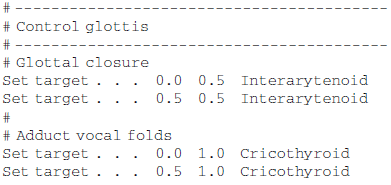
\includegraphics{resources/praatScript.png} 
\end{center}
\caption{Example of Praat script to set two variables. Source : \cite{ref5}}
\label{praatScript}
\end{figure}

If each parameter get two value, it makes a lot of value to define and a heavy object to manipulate. Fortunately, Praat will automaticly complete the values for some parameters by default, we will only have to define the 10 most important.

It means that the structure we will make evolve int the GA is a structure containing 20 values, one for each parameter to set in the Praat script.

\subsection{Evolution Operators and population}
We use two common evolution operators for a GA : a one point cross over at each generation and then a mutation with a probability of 0.2 to append.

\paragraph*{}
The population we make evolve is composed of 10 individuals, It is sufficient for the moment.

\subsection{Ending conditions}
We have three possible ways to stop the algorithm. 
\begin{enumerate}
\item We can define a matching value in the fitness function that he might reach.
\item We can define an execution time and get the better solution at this time.
\item We can define a maximum generation number and get the value at this time.
\end{enumerate}

For the moment, the algorithm work with the first option and try to reach the value that correspond to the 
perfect matching. We will adapt it in the future versions according to the time necessary to find a solution and the quality of the solutions find.

\section{Particularities}

\subsection{In the sequence generation}
The first point about the particularities is that we have a knowledge of how the speech synthesis work and we have an idea of the range of values for each parameter. It allow to use this knowledge to restrain the search domain without making the GA deterministic.

It is very important in term in performance because some values can be fix and Praat use a range of value for each parameter so it useless to try to get out of this interval.

\subsection{In the fitness function}
The second point is that I use another program (Praat) to execute a script in the fitness function. This script will generate a sound, analyse it to get the formants and then get the values back. Then I will compare the formant in the result from Praat with the formants given to the program as the target.

It is different from other fitness function that typically take care themselves of the calculation part. Here it delegate it to another program and only do a comparison.
It do it for each individual of the generation's population.

\paragraph*{}
The third point is that I adapt the fitness function to be flexible. The formants values used as target are just a reference, they are not an exact value to reach. In practice, we can estimate that a formant value can increase or decrease over 10\% of this value. That's why the fitness function of my GA compare the values of the formants of the candidate and accept a value in the interval of +/-10\% of the values of the target's formants.

\section{Recap}
We have seen that the structure of my GA respect the general structure of a common GA with some particularities to adapt to the subject of speech synthesis.

As a recap, here is the algorithm :


\begin{verbatimtab}[3]
1) generate the candidate population with the reduced range values.
2) while not converge{
		a) For each individual of the population{
					-> generate Praat's script with values 
					-> make it executed by Praat
					-> get the formant values of generated sound back
					-> compare with the formants values of the target sound	   
		   }endFor
		   
		b)if no solution found then{ 
				cross over and mutation to get an evolved population.
			}else{
				 quite the while loop  	 
			}   
		
   }endWhile

\end{verbatimtab}

\chapter{How to connect Java and Praat}
Giving the Praat's API, we need to use two different ways to connect Java and Praat.
We need to consider one way to communicate between Java and Praat and another way to communicate from Praat to Java.
The first one is use to send and execute the Praat script and the second to send the answer from Praat to Java. They both use a different techniques to be executed and so a particular treatment must be done for each.

\section{From Java to Praat}
We want to send a Praat's script to Praat and have it executed. The way I choose is the software SendPraat. It is a program developed by the same authors as Praat and available at this address : \url{http://www.fon.hum.uva.nl/praat/sendpraat.html}. It allow to send orders to a {\bfseries running instance of Praat}\footnote{This is very important, if there is no Praat already launched, SendPraat won't work.}.

\paragraph*{}
It means we need two programs :

\begin{enumerate}
\item A normal Praat software already launched.
\item SendPraat which will give it orders. No need to launch this one, it only works in command line.
\end{enumerate}

If you give SendPraat the name of a script, it will made Praat launch and execute it. The only thing left is to make Java executed SendPraat. For this, I used the Java Runtime Environment which can use the command line of windows. I will explain it in the second part of this report.

\paragraph*{}
Note : I use a SendPraat.exe as I am a windows user but you can compile the source code yourself to use it in your own operating system. If you want to make Praat communicate with a C program, you can use the SendPraat directive, no need to compile source code. For more information, look at the Praat's API, section Praat scripting. As I was working in Java, the solution I presented is currently the best.

\section{From Praat to Java}
There is only one way to make Praat communicate with another program, whenever the language is: the sockets\footnote{It only work for windows and Linux, it is the Praat API which manage it like this.}. 

\paragraph*{}
Sockets are tools used in computer science to make two different program communicated. For this, they will use the network principles and send network packets to a computer on a specified port. It is not necessary that the target is running on another computer, it can be the same and int that case, we use a local network call localhost. The first program will send a message to the other specifying the port and the second one will listen will listen to the port and get the message when it arrived.

\paragraph*{}
Praat allows to send sockets by the directive "sendsocket" but it cant received sockets from another program. That is why we got to use the SendPraat program in the other side.
If Praat send a socket then our GA will need a functionality which always listen to this port and  will take the message. Such functionality basically call a {\bfseries Server}.
In that purpose, I implemented a Java server that listen to a specific port to get the message from Praat. I will describe it in the second part of the report.

\section{Sequencing}
There is a problem of sequencing to take care to synchronise Java and Praat. The problem came from the fact that they are two different thread(program) running.
They both have a different execution's speed. The Java's GA work very fast, each generation take a few seconds while each sound synthesis take a few seconds in Praat. For example, it take approximately 12 second to Praat to generate a 2.0 seconds sound. So there is a problem of speed and synchronisation.

\paragraph*{}
This is why I should have establish a sequencing order between the two programs to force the Ga to wait for Praat's answer before going to the next individual. More precisely, to wait for the server to get the answer from Praat and store it into the GA. The GA could do the comparison of formants while it is done.

\paragraph*{}
The only solution was to use semaphores. It is a computing technique for sequencing tasks. It work on the principle of token. You have a token in a box, if someone want to do an action he took the token and it released it when finished. The others wait for the token to be free before doing their action.

\paragraph*{}
I used in fact two levels of semaphore in the fitness function :


\paragraph*{}
The first on is when the GA start the fitness function, it took the token and it released it when it had finished the comparison and calculated a matching mark. It prevent the Ga to launch the fitness function with another candidate while still running the previous one. For example if Praat is still running a synthesis, it wont be able to do the comparison with a empty values and switch to the next candidate.

\paragraph*{}
The second level is in the function fitness itself, it allow to be sure that the server had store the message into the GA. As the server is a different thread, it is a obligation. It forbid the fitness function to do the comparison with the reference formant until a value was set by the server. It avoid errors.

\paragraph*{}
Here is the representation in the form of a algorithm. The operations concerning the semaphores are written with letters whereas the other actions are written with numbers
\begin{verbatimtab}[3]
fitness function{
	A) launch of the function, took the token "function" to avoid the GA to launch the next one until 		   this one is finish. The token "praat result stored" is also locked.
		1) create a script with the candidates values
		2) send it to praat
		3) praat execute the script and calculate the formant values 
		4) the server get the socket and store the result
			=> release the "praat result stored" token
		
		B) If the token "praat result stored" is available we can continue, else we wait until it is 		available.
			5) compare the formants values
			6) give a matching result
	C) release the token "function".
}
\end{verbatimtab}

\section{Recap}
So in conclusion we had to consider two different side for the communications:
\begin{itemize}
\item The message from Java to Praat. On this side, we had to use a specific Praat's like program call SendPraat.
\item And a message and the message from praat to Java where we had to use a Java's Server to listen to Praat's sockets.
\end{itemize}


The figure below show how it works :
\begin{figure}
\begin{center}
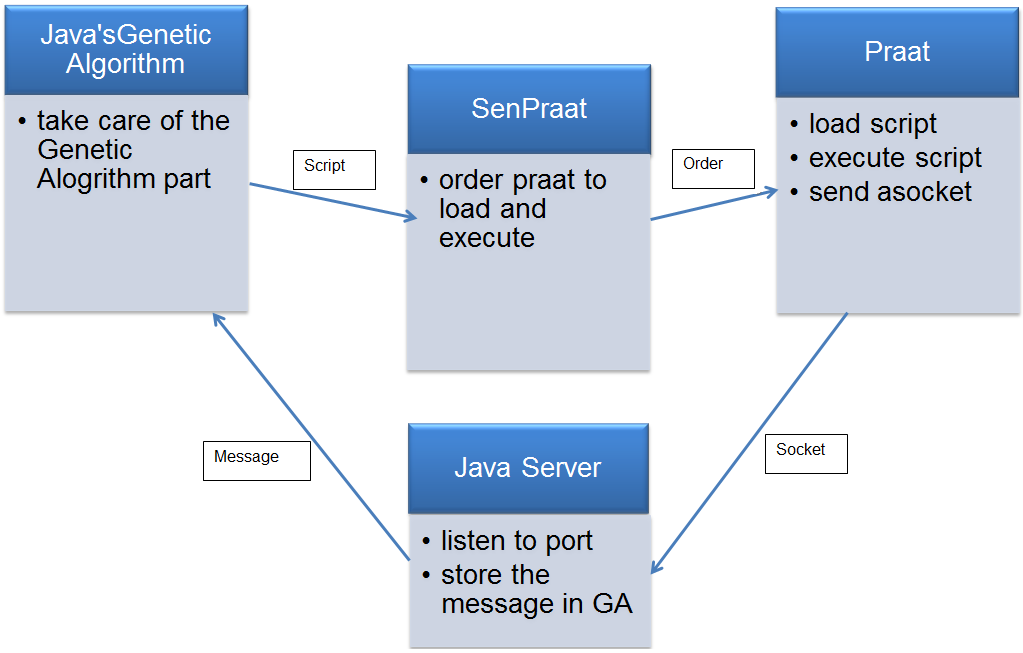
\includegraphics[scale=0.6]{resources/architecture.png} 
\end{center}
\caption{The exchange of information between Java and Praat and the role of each entity}
\label{architecture}
\end{figure}

\part{Implementation Details}

\chapter{the GA}

\section{watchmaker}
In this project, I used the Watchmaker's Genetic Algorithm API\cite{ref}. It is an Java API which provided all the objects and methods to run a genetic Algorithm. The only thing I had to do is reimplemented some classes to use my own objects and operations as cross over, mutation, ... but all the structure of the GA behind was already defined.

\section{basics elements to manipulate}
I will present here the classes containing the basics elements i manipulated to use the GA.
I will make a short presentation to explain what the elements are designed for and how to use them in the project perspective. I wont make a technical explanation of each. I have already written a Java documentation for that purpose which is available at : \url{https://github.com/phervo/ProjetEte2013/tree/master/doc}

\subsection{The Alphabets}
The class Alphabet is a class which allow to define an interval of value for one or several Praat parameters.
The goal is to have a interval of possible for each parameter.
For the moment I have  special Alphabets for masseter and Lungs. All the other parameters shared the same alphabet call otherAlphabet but it could be possible to declare new alphabets. All the alphabets are gathered in a meta-alphabet called GlobalAlphabet. It is the alphabet that will be use by the GA.

\paragraph*{}
If you want to introduce a new alphabet, proceed as follow :
\begin{enumerate}
\item Create a new Alphabet in the GlobalAlphabet Class with the getters and setters you need.
\item Modify the functions in MessageToPraat to use your alphabet where it is needed.
\end{enumerate}

\subsection{the Sequence}
The class Sequence represent the 20 values I have presented in \ref{Thecandidate} page \pageref{Thecandidate}. It will be the structure of the candidates values, the structure which will evolve during the GA. We are not suppose to instantiate it directly, the SequenceFactory of the GA will do it for us.

\subsection{the formants}
I build a special structure for the formants. The structure of a formant itself is defined in the Formant class. You can modify it here if you want to change the structure. Then I defined in FormantSequence the structure of the formants I will analyse : two formants. It is this class that you should manipulate if you just want to use the formants and not the other. I created a special constructor in which you can give a vowel letter. It will automaticly create the formant with the values corresponding to the vowel. For the moment I only implemented it for "i" but in the future i will add others. It can be useful to specify the target for example.

\subsection{the script}
I generate a script with a template file and the values of the candidate Sequence. The templates are stored in the MessageToPraat class. They aren't written as a file in the disk because it is too long to procede. Instead, they are store in the central memory of the computer to be faster.

\section{The run}
The run of the GA is done according to the watchmaker API. I wrote all the orders in a class called GeneticAlgorithmCall. The only thing it need to know is the length of the sequence we wanted to manipulate.

\chapter{the communication}
\section{SendPraat}
To run the program you need to have sendPraat installed and a running instance of Praat.
I created a function to open and close Praat and another to send it an order using sendPraat. All these functions are available in the Communication package. It work using the Java runtime environment which allow to use the command line. Each call create a new process but i add a special parameter to told the program to wait for the full execution of the process before continuing so there is no need of semaphore here.

\section{the Server}
As I said in the overAll, i implemented a server to listen to the Praat's sendsocket port.
I design it as a thread to be sure that it will listen all the time without blocking the execution of the GA. When it get a message it store it in the Ga specified in parameter during the construction. I separate
the Ga and the Server to allow it to be use in another application using praat if necessary, you just add to modify a little the run method. 

\paragraph*{}
As the program is always listening and that is all, you had to manage to close it in a specific method elsewhere.
I put it in the CloseServer class. It might be use once the Ga has finish and found a solution.

\chapter{Performance and result}

\section{code}
Here is the only code you had to use to run my Java Application. All in 7 lines :

\begin{lstlisting}
OrderToPraat.launchPraat();
OrderToPraat.sendMessageToPrat(MessageToPraat.writePraatScriptHeader());
GeneticAlgorithmCall ga= new GeneticAlgorithmCall(19); //init
ServerThread.getInstance(ga);
ga.startAlgorithm();
CloseServer.envoyerMessageFermeture();
OrderToPraat.closePraat();
\end{lstlisting}

The first and the last line launch and close praat, the last one is optional.
The second line create the Praat's speaker and artword.
The third line initiale a genetic algortihm object. It is launch in the fifth line using the startAlgorithm method.
As I explain in this report, I designed the server independent from the GA. So you have to get one from the ServerThread.getInstance method line 4.
We close it at the end of the execution, line 7, using the specific method dedicated to this task or it will continue to run.

\section{result}
At the end of the run, my application generate a Praat script with the result values.
You just have to load it in Praat to listen it.

\listoffigures

\bibliographystyle{alpha} 
\bibliography{bib} % mon fichier de base de données s'appelle bib.bib
\end{document}